%!TEX root = ../Diploma.tex


\begin{section}{Описание методологии}
   В этой главе будет дано описание начального набора данных,
   его предабработка, признаки, которые были использованы для построения классификатора, а также описание использовавшихся алгоритмов.
  \begin{subsection}{Набор данных}
    \label{sec:dataset}
    Наличие размеченной коллекции твитов в задаче классификации
    спама имеет критически важное значение.
    Набора данных, который бы полностью удовлетворял всем требованиям найдено не было.
    В качестве базы был использован набор данных из \cite{Lee}, который распространяется
    по открытой некоммерческой лицензии Creative Commons.
    Датасет представляет из себя случайно собранную в период с 30.11.2009 г. по 02.08.2010 г. информацию
    о 22,223 спамерах и 19,276 легитимных пользователях, а также 2,353,473 и 3,259,693
    спамовых и легитимных сообщениях этих аккаунтов соответственно.
    Данные были получены путем регистрации 60 аккаунтов-приманок для спама, целью которых
    было иммитировать пользовательское поведение.
    Аккаунт-приманка имел возможность совершать одно из 4-х действий: (1) Пубиковать обычное текстовое сообщение (2) Упоминать один из других аккаунтов-приманок с помощью символа <<@>>  (3) Публиковать сообщение, содеражащее ссылку (4) Публиковать сообщение, содержащее одну из ТОП-10 трендовых слов Twitter
    Каждый из аккаунтов-приманок не мог взаимодействовать
    с пользователями не из круга других аккаунтов-приманок. Как только один из искуственных аккаунтов упоминался в сообщении аккаунта <<извне>> или появлялся у него в подписках, информация о новом спамовом аккаунте заносились в датасет.


  \end{subsection}

  \begin{subsection}{Предобработка данных}
     Перед извлечением признаков из набора данных к тексту твитов были применены несколько техник предобработки с целью нормализации и уменьшения <<шума>> на стадии классификации.
     Также для извлечения семантических признаков из текста твита игнорировались ссылки, хештеги и упоминания.
  \end{subsection}

  \begin{subsection}{Описание признаков}
    Поскольку спамеры и обычные пользователи имеют различные цели при размещении твитов или взаимодействии с другими пользователями в Twitter, справедливо предположение, что характеристики спам-твитов сильно отличаются от обычных твитов.
    Признаки, присущие твиту, включают, помимо самого твита, набор метаданных, включая информацию о пользователе, разместившем твит, который также легко доступен в потоке твитов, к которому у нас есть доступ.
    Анализу подвергается широкий спектр признаков, которые не требуют больших вычислительных затрат, а также описывают лингвистические свойства, которые могут извлекаться из текста твита.
    Признаки были разделены по следующим группам:
    \begin{enumerate}
      \item Пользовательские признаки
      \item Признаки контента
      \item N-граммы
      \item Сентимент-признаки
    \end{enumerate}

    \textbf{Пользовательские признаки} включают в себя список из 11 атрибутов об авторе твита (см. Таблицу \ref{tab:features}), который генерируется из метаданных каждого твита, таких как репутация пользователя \cite{Wang} (см. Рис \ref{pic:reputation}), который определяется как соотношение между числом подписчиков к а общему числу подписчиков и подписок и используется для измерения степени влиятельности пользователя. Такие признаки как число ретвитов не использовались, поскольку они содержат в себе историчность.

    \begin{figure}[ht!]
    \centering
    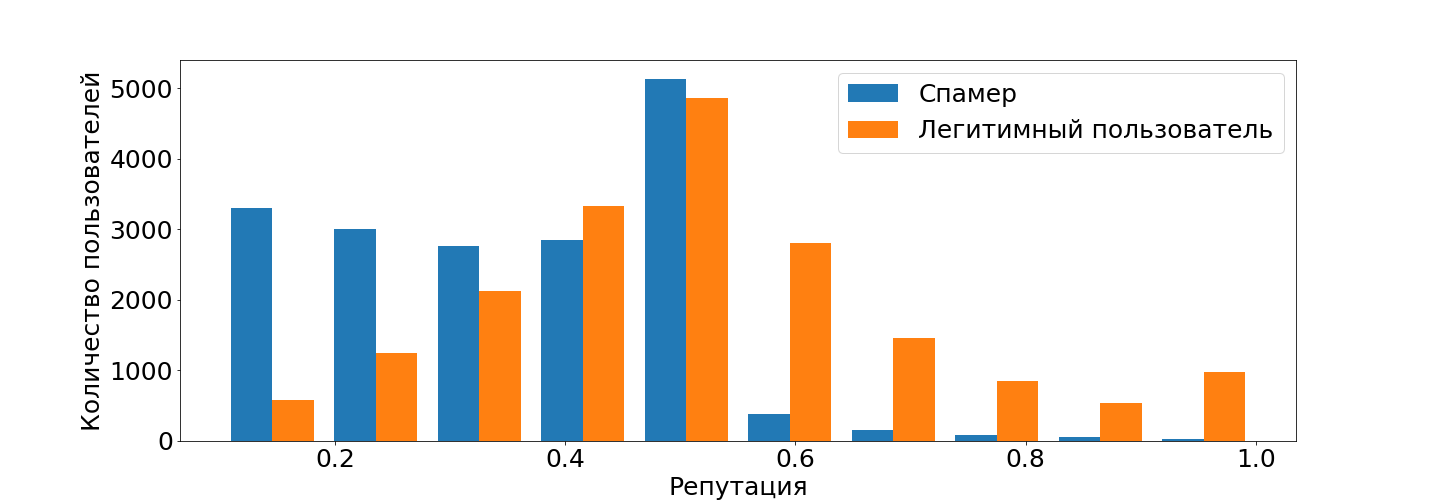
\includegraphics[width=1.0\textwidth]{pics/reputation}
    \caption{Распределение пользователей по репутации Twitter}
    \label{pic:reputation}
    \end{figure}

    \textbf{Признаки контента} фиксируют лингвистические свойства текста каждого твита (табл. \ref{tab:features}), включая список атрибутов контента и тегов части речи.
     Среди 17 контентных атрибутов присутствует количество спам-слов и количество спам-слов на одно слово, которые генерируются путем сопоставления с известными спамовыми словами \footnote{https://github.com/splorp/wordpress-comment-blacklist/blob/master/blacklist.txt}.
     Распознавание части речи (part-of-speech или POS) обеспечивает
     синтаксическую (или грамматическую) информацию о предложении и
     был использован в сообществе обработки естественного языка для оценки текстовой информативности (например, \ref{Tan} использовали подсчеты POS как показатель информативности для твитов). Я использовл тэггер для работы с Твиттером \cite{Gimpel}, и признак POS состоит из униграмма и 2-skip-bi-gram представления тегов POS для каждого твита, чтобы уловить структуру и, следовательно, информативность текста.

     \textbf{N-граммы}
     Модели N-грамма уже давно используются в обработке естественного языка для выполнения самых различных задач, включая текстовую классификацию. Хотя он часто подвергается критике за отсутствие какого-либо явного представления долгосрочной или семантической зависимости, он удивительно эффективен для простой текстовой классификации с разумным количеством данных обучения. Для того, чтобы дать лучший результат классификации при вычислительной эффективности, был использован uni + bi-gram или bi + tri-gram с двоичными данными (т.е. 1 при присутствии признака, и 0 при отсутствии), term-frequency (tf) и tf- Idf (т.е. Частота терминов, умноженная на обратную частоту документа).

     \textbf{Сентимент-признаки}
     Феррара \cite{Ferrara} использовал сентимент-признак на уровне текста твита как часть признакового описания обьекта. Я использовал тот же список лексиконов из \cite{Mohammad} (который отлично показал себя на Semeval-2014 Task 9 для анализа настроений в Twitter) для генерирования наших характеристик настроения, включая вручную созданные лексиконы чувств: лексикон AFINN \cite{Nielsen} , Лексикон Bing Liu \cite{Liu}, лексикон MPQA [19]; И автоматически сгенерированные лексиконы чувств: лексика чувственного восприятия Hashtag NRC [13] и лексика Sentiment140 [13].

     \begin{table}[H]
     \centering
     \resizebox{\textwidth}{!}{\begin{tabular}{|l|l|l|l|}
     \hline
     \textbf{Пользовательские признаки} & \textbf{Признаки контента} & \textbf{N-граммы} & \textbf{Сентимент-признаки} \\
     \hline
     Длина названия профиля & Количество слов (КС) & Uni + bi-gram or bi + tri-gram & Автоматически созданный сентимент-лексикон \\
     \hline
     Длина описания профиля & Количество символов &&  Созданный вручную сентимент-лексикон \\
     \hline
     Количество подписок (ПС) & Количество пробелов &&\\
     \hline
     Количество подписчиков (ПЧ) & Количество слов с заглавной буквы (КЗ) &&\\
     \hline
     Количество твитов & КЗ/КС   &&\\
     \hline
     Количество твитов &  Максимальная длина слова  &&\\
     \hline
     <<Возраст>> аккаунта, ч. (ВА) & Средняя длина слова &&\\
     \hline
     Соотношение подписчиков и подписок (ПЧ/ПС) & Количество символов <<!>> &&\\
     \hline
     Репутация пользователь (ПЧ/(ПС + ПЧ))) & Количество символов <<?>> &&\\
     \hline
     Прирост подписок (ПС/ВА) & Количество URL (КЛ) &&\\
     \hline
     Количество твитов в день & КЛ/КС &&\\
     \hline
     Количество твитов в неделю & Количество хэштегов (КХ) &&\\
     \hline
    & КХ/КС &   &\\
     \hline
    & Количество упоминаний (КУ) &&\\
     \hline
    & КУ/КС &&\\
     \hline
    & Количество спамовых слов (КСП) &&\\
     \hline
    & КСП / КС &&\\
     \hline
    & Тэг части речи &&\\
     \hline
     \end{tabular}}

     \caption{Список итоговых признаков}
     \label{tab:features}
     \end{table}
  \end{subsection}

  \begin{subsection}{Используемые классификаторы}

    Наиболее популярным и эффективным подходом на данный момент является использование машинного обучения с учителем с различными признаками, основанными как на содержании сообщений, так и на свойствах отдельных профилей пользователей.

    Машинное обучение (machine learning) – это область научного знания, имеющая дело с алгоритмами, <<способными обучаться>>. Необходимость использования методов машинного обучения объясняется тем, что для многих сложных – <<интеллектуальных>> – задач (например, распознавание рукописного текста, речи и т. п.) очень сложно (или даже невозможно) разработать <<явный>> алгоритм их решения, однако часто можно научить компьютер обучиться решению этих задач. Одним из первых, кто использовал термин <<машинное обучение>>, был изобретатель первой самообучающейся компьютерной программы игры в шашки А. Л. Самуэль в 1959 г. \cite{Samuel}. Под обучением он понимал процесс, в результате которого компьютер способен показать поведение, которое в нее не было заложено <<явно>>. Это определение не выдерживает критики, так как не понятно, что означает наречие "явно". Более точное определение дал намного позже Т. М. Митчелл \cite{Mitchell}: говорят, что компьютерная программа обучается на основе опыта $E$ по отношению к некоторому классу задач $T$ и меры качества $P$, если качество решения задач из $T$, измеренное на основе $P$, улучшается с приобретением опыта $E$.

    В настоящее время машинное обучение имеет многочисленные сферы приложения, такие, как компьютерное зрение, распознавание речи, компьютерная лингвистика и обработка естественных языков, медицинская диагностика, биоинформатика, техническая диагностика, финансовые приложения, поиск и рубрикация текстов, интеллектуальные игры, экспертные системы и др.


    На этапе классификации и оценки были протестированы 5 алгоритмов классификации, реализованных с использованием scikit-learn\footnote{http://scikit-learn.org/}: Наивный Байесовский классификатор,
    Метод \textit{k} ближайших соседей, метод опорных векторов (SVM), решающее дерево, случайные леса.

    \begin{subsubsection}{Наивный Байесовский классификатор}

Идея Байесовского классификатора для спам-фильтра основана на предположении,
что некоторые слова особенно часто встречаются в спаме. Отсюда возникает идея посчитать для каждого слова $w$ из коллекции текстов количество писем с ним $n_{ws}$
в спаме (spam) и количесвто писем с ним $n_{wh}$ в <<не спаме>> (ham), а затем оценить вероятность появления каждого слова $w$ в спамном и неспамном тексте:

\begin{equation}
  P(w|spam) = n_{ws}/n_s; P(w|ham) = n_{wh}/n_s;
\end{equation}

Получив текст письма, для которого нужно определить, относится оно к спаму или нет, мы можем оценить вероятность появления всего текста в классе <<спам>> и в классе <<не спам>> произведением вероятностей слов:
\begin{equation}
P(text|spam) = P(w_1|spam)P(w_2|spam)...P(w_N|spam)
\end{equation}
\begin{equation}
P(text|ham) = P(w_1|ham)P(w_2|ham)...P(w_N|ham)
\end{equation}

<<Наивность>> подхода в этом случае состоит в предположении, что вхождение разных слов в текст – это независимые события.

Получив текст письма, для которого нужно определить, относится оно к спаму или нет, мы можем выбрать тот класс, в котором вероятность возникновения этого текста больше:
\begin{equation}
a(text) = argmax P(y|text)
\end{equation}
\end{subsubsection}

    \begin{subsubsection}{Метод \textit{k} ближайших соседей}

      Метод \textit{k} ближайших соседей (\textit{k} nearest-neighbor, k-NN) относится к наиболее простым и в то же время универсальным методам, используемым как для решения задач классификации, так и восстановления регрессии. В случае классификации новый объект классифицируется путем отнесения его к классу, являющемуся преобладающим среди \textit{k} ближайших (в пространстве признаков) объектов из обучающей выборки. Если \textit{k} = 1, то новый объект относится к тому же классу, что и ближайший объект из обучающей выборки.

      Аналогичный способ используется и в задаче восстановления регрессии, с той лишь разницей, что в качестве ответа для объекта выступает среднее ответов \textit{k} ближайших к нему объектов из обучающей выборки.

      Опишем метод более формально. Пусть $N_k(x)$ - множество $k$ ближайших к $x$ объектов из обучающей выборки. Тогда для задачи классификации положим

      \begin{equation}
        f(x)=arg⁡min_{y}⁡|\{i\colon y^{(i)}=y, x^{(i)} \in N_k (x)\}|
      \end{equation}

      а для задачи восстановления регрессии –

      \begin{equation}
      f(x)=\frac{1}{k} \sum_{x^{(i)} \in N_k(x)}y^{(i)}
     \end{equation}

     В некоторых случаях данные ответы учитываются с весами, обратно пропорциональными расстоянию до объекта. Это особенно полезно для решения задачи классификации с несбалансированными данными, т. е. когда число объектов, относящихся к разным классам, сильно различно.

Для определения ближайших соседей обычно используется евклидово расстояние:

    \begin{equation}
      p(x,x') = \sqrt{\sum\limits_{j=1}^d |x_j - x'_j|^2}
    \end{equation}


    однако оно применимо только для признаков, описываемых количественными переменными. Если все переменные качественные, то можно использовать расстояние Хэмминга:

    \begin{equation}
      p(x,x') = \sum\limits_{j=1}^d I(x_j \neq x'_j)
    \end{equation}

    В общем случае используют функцию:

\begin{equation}
  p(x,x')=\sum\limits_{j=1}^d a_j p_j (x_j,x'_j)
\end{equation}

    где $a_j$ – неотрицательные параметры,$p_j(x_j,x'_j)=(x_j-x'_j)^2$  для количественных переменных, $p_j(x_j,x'_j)=I(x_j \neq x'_j)$  для качественных переменных. Заметим, что функция расстояния не обязательно должна быть метрикой и неравенство треугольника может быть не выполнено.
Для повышения точности модели также могут использоваться специальные алгоритмы обучения метрики расстояния (например, Large Margin Nearest Neighbour \cite{Weinberger}).
Одним из основных параметров, влияющих на обобщающую способность алгоритма, является число <<ближайших соседей>>  $k$. В целом, выбор определенного значения обусловлен характером данных задачи. Большие значения $k$ могут привести как к более точному описанию границы, разделяющей классы, так и переобучению. Обычно для выбора $k$ применяют различные эвристики, в частности, метод перекрестного контроля.

    \end{subsubsection}

    \begin{subsubsection}{Метод опорных векторов (SVM)}

      Один из самых популярных методов машинного обучения – машина опорных векторов (SVM – Support Vector Machine) – является развитием идей, предложенных в 1960–1970 гг. В. Н. Вапником и А. Я. Червоненкисом. Окончательное очертание метод принял в 1995 г., когда было показано, как в этом методе можно эффективно использовать ядра \cite{Cortes}.
Данный метод изначально относится к бинарным классификаторам, хотя существуют способы заставить его работать и для задач мультиклассификации.
Идею метода удобно проиллюстрировать на следующем простом примере: даны точки на плоскости, разбитые на два класса (Рисунок \ref{pic:SVM1}).

  Проведем линию, разделяющую эти два класса. Далее, все новые точки (не из обучающей выборки) автоматически классифицируются следующим образом:
точка выше прямой попадает в класс A,
точка ниже прямой — в класс B.

\begin{figure}[ht!]
\centering
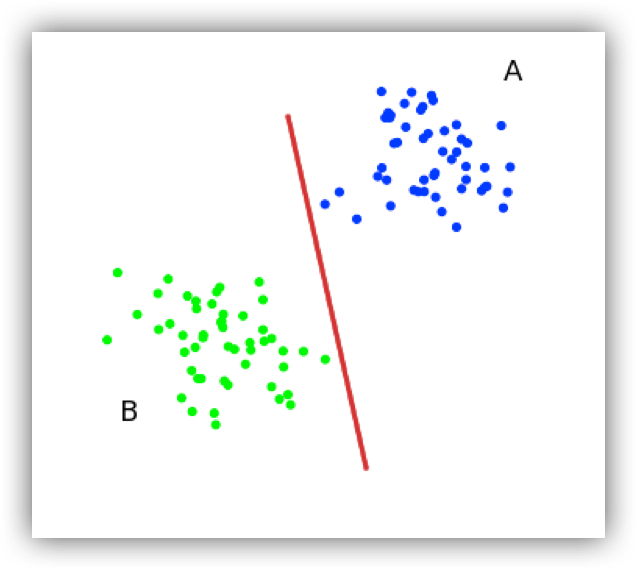
\includegraphics[width=0.4\textwidth]{pics/SVM1}
\caption{Демонстрация метода опорных векторов}
\label{pic:SVM1}
\end{figure}

Такую прямую назовем разделяющей прямой. Однако в пространствах высоких размерностей прямая уже не будет разделять наши классы, так как понятие «ниже прямой» или «выше прямой» теряет всякий смысл. Поэтому вместо прямых необходимо рассматривать гиперплоскости — пространства, размерность которых на единицу меньше, чем размерность исходного пространства. В $\mathbb{R}^3$, например, гиперплоскость — это обычная двумерная плоскость.
В нашем примере существует несколько прямых, разделяющих два класса (Рисунок \ref{pic:SVM2}):

\begin{figure}[ht!]
\centering
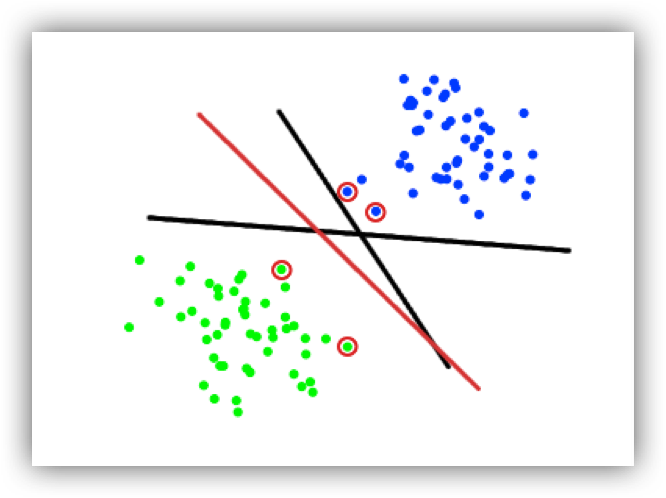
\includegraphics[width=0.4\textwidth]{pics/SVM2}
\caption{Демонстрация метода опорных векторов}
\label{pic:SVM2}
\end{figure}

С точки зрения точности классификации лучше всего выбрать прямую, расстояние от которой до каждого класса максимально. Другими словами, выберем ту прямую, которая разделяет классы наилучшим образом (красная прямая на рис. \ref{pic:SVM2}). Такая прямая, а в общем случае — гиперплоскость, называется оптимальной разделяющей гиперплоскостью.
Другими словами, оптимальной разделяющей гиперплоскостью называется гиперплоскость, ортогональная отрезку, соединяющему ближайшие точки выпуклых оболочек двух классов, и проходящая через середину этого отрезка.

Вектора, лежащие ближе всех к разделяющей гиперплоскости, называются \textit{опорными векторами} (support vectors). На Рисунке \ref{pic:SVM2} они помечены красными кружочками.

Для дальнейшей формализации положим в математической постановке задачи обучения с учителем,$\mathbb{Y} = \{-1,1\}, \mathbb{X} = \mathbb{R}^n$ .
Рассмотрим случай линейной разделимости. Пусть имеется обучающая выборка: $(x_1,y_1 ),…,(x_m,y_m ),x_i \in \mathbb{R}^n,y_i \in \{-1,1\}$.
Метод опорных векторов строит классифицирующую функцию  в виде
\begin{equation}
  f(x)=sign (w \times x + b)
\end{equation}
где $w \times x$ — скалярное произведение, $w$  — нормальный вектор к разделяющей гиперплоскости,$b$  — вспомогательный параметр. Те объекты, для которых $f(x) = 1$ попадают в один класс, а объекты с $f(x) = -1$ — в другой. Выбор именно такой функции неслучаен: любая гиперплоскость может быть задана в виде $w \times x + b = 0$ для некоторых $w$ и $b$.

Далее, мы хотим выбрать такие $w$ и $b$ которые максимизируют расстояние до каждого класса. Можно подсчитать, что данное расстояние равно $\frac{1}{||w||}$ (Рисунок \ref{pic:SVM3}) Проблема нахождения максимума $\frac{1}{||w||}$ эквивалентна проблеме нахождения минимума $||w||^2$. Запишем все это в виде задачи оптимизации:
\begin{equation}
  \begin{cases} arg⁡min_{(w,b)⁡} ||w||^2 , \\ y_i (w \times x+b) \geq 1, i=1,…,m \end{cases}
\end{equation}


которая является стандартной задачей квадратичного программирования и решается с помощью множителей Лагранжа.

\begin{figure}[ht!]
\centering
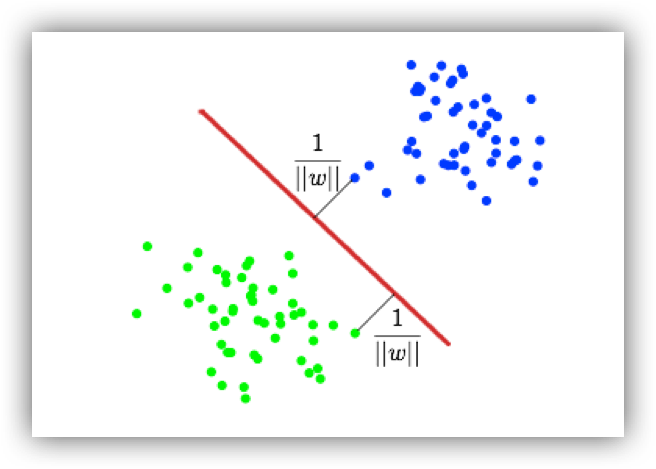
\includegraphics[width=0.4\textwidth]{pics/SVM3}
\caption{Демонстрация метода опорных векторов}
\label{pic:SVM3}
\end{figure}

На практике случаи, когда данные можно разделить гиперплоскостью, или, как еще говорят, \textit{линейно}, довольно редки. Пример линейной неразделимости можно видеть на Рисунок \ref{pic:SVM4}

\begin{figure}[ht!]
\centering
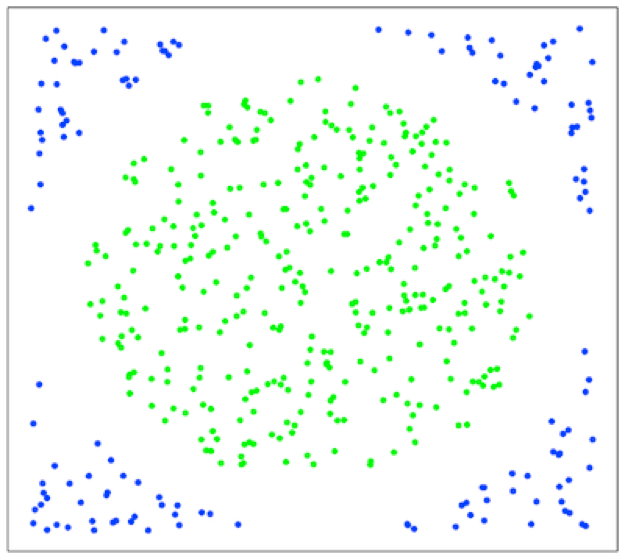
\includegraphics[width=0.4\textwidth]{pics/SVM4}
\caption{Демонстрация метода опорных векторов}
\label{pic:SVM4}
\end{figure}

В этом случае поступают так: все элементы обучающей выборки вкладываются в пространство $\mathbb{Z}$ более высокой размерности с помощью специального отображения $\varphi:\mathbb{R}^n \rightarrow Z$. При этом отображение  выбирается так, чтобы в новом пространстве $Z$ выборка была \textit{линейно} разделима.
Классифицирующая функция $f$ принимает вид
\begin{equation}
  f(x)=sign (w \times \varphi(x)+b)
\end{equation}
Выражение $K(x,x')= \varphi(x)\times \varphi(x')$ называется \textit{ядром} классификатора. С математической точки зрения ядром может служить любая положительно определенная симметричная функция двух переменных. Положительная определенность необходимо для того, чтобы соответствующая функция Лагранжа в задаче оптимизации была ограничена снизу, т.е. задача оптимизации была бы корректно определена. Точность классификатора зависит, в частности, от выбора ядра.
Чаще всего на практике встречаются следующие ядра:
\begin{enumerate}
  \item Полиномиальное: $K(x,x')= (x \times x'+ const)^d$
  \item Радиальная базисная функция: $K(x,x')= e^{-\gamma|x-x'|^2},\gamma > 0$
  \item Гауссова радиальная базисная функция: $K(x,x')= e^{-\frac{|x-x'|^2}{(2\sigma^2)}}$
  \item Сигмоид:$K(x,x') = \tanh⁡(k(x\times x')+c), k > 0, c < 0$
\end{enumerate}


Для того чтобы использовать метод опорных векторов для задачи классификации с числом классом $N > 2$, возможно также использовать следующие стратегии:
\begin{enumerate}
  \item "Каждый против каждого": построить $N(N-1)/2$ классификаторов на всех возможных подзадачах бинарной классификации. Новый объект классифицируется всеми построенными решающими правилами, затем выбирается преобладающий класс.
  \item "Один против всех": обучить $N$ моделей на задачах бинарной классификации вида "один класс против всех остальных". Класс нового объекта выбирается по максимальному значению отступа.
\end{enumerate}

    \end{subsubsection}

    \begin{subsubsection}{Метод решающего дерева}
Метод деревьев решений (decision trees) является одним из наиболее популярных методов решения задач классификации и прогнозирования. Иногда этот метод Data Mining также называют деревьями решающих правил, деревьями классификации и регрессии.

Как видно из последнего названия, при помощи данного метода решаются задачи классификации и прогнозирования.
Основная идея деревьев решений состоит в рекурсивном разбиении пространства признаков с помощью \textit{разбиений} (\textit{splits}) гиперплоскостей, параллельных координатным гиперплоскостям (если признак – количественный), либо по категориям (если признак номинальный). В каждом из полученных в конце процедуры "ящиков" $R_1,R_2,…,R_M$ функция аппроксимируется константой.

Впервые деревья решений были предложены Ховилендом и Хантом (Hoveland, Hunt) в конце 50-х годов прошлого века. Самая ранняя и известная работа Ханта и др., в которой излагается суть деревьев решений - "Эксперименты в индукции" ("Experiments in Induction") – была опубликована в 1966 году.

В наиболее простом виде дерево решений – это способ представления правил в иерархической, последовательной структуре. Основа такой структуры – ответы "Да" или "Нет" на ряд вопросов. В этом случае решается задача бинарной классификации, т.е. создается дихотомическая классификационная модель, или, так называемые, бинарные деревья.

В узлах бинарных деревьев ветвление может вестись только в двух направлениях, т.е. существует возможность только двух ответов на поставленный вопрос ("да" и "нет"). Бинарные деревья являются самым простым, частным случаем деревьев решений. В остальных случаях, ответов и, соответственно, ветвей дерева, выходящих из его внутреннего узла, может быть больше двух.

Как правило, внутренние узлы дерева являются атрибутами некой базы данных (или признаками). Эти атрибуты называют прогнозирующими, или атрибутами расщепления (splitting attribute). Конечные узлы дерева, или листы, именуются метками класса, являющимися значениями зависимой категориальной переменной.

Каждая ветвь дерева, идущая от внутреннего узла, отмечена предикатом расщепления. Последний может относиться лишь к одному атрибуту расщепления данного узла. Характерная особенность предикатов расщепления: каждая запись использует уникальный путь от корня дерева только к одному узлу-решению. Объединенная информация об атрибутах расщепления и предикатах расщепления в узле называется критерием расщепления (splitting criterion).

Для любой задачи может быть построено множество деревьев решений различного качества, с различной прогнозирующей точностью.

Качество построенного дерева решения весьма зависит от правильного выбора критерия расщепления. Над разработкой и усовершенствованием критериев работают многие исследователи.

Преимущества деревьев решений:
\begin{enumerate}
  \item Возможность производить обучение на исходных данных без их дополнительной предобработки (нормализация и т. п.);
  \item Не требуют от пользователя выбора входных атрибутов (независимых переменных)
  \item Нечувствительность к монотонным преобразованиям данных;
  \item Устойчивость к выбросам;
  \item Возможность обрабатывать данные с пропущенными значения;
  \item Поддержка работы с входными переменными разных (смешанных) типов (и с числовыми, и с категориальными типами данных);
  \item Позволяют создавать классификационные модели в тех областях, где аналитику достаточно сложно формализовать знания;
  \item Возможность интерпретации построенного дерева решений (его интуитивность);
  \item Точность моделей, созданных при помощи деревьев решений, сопоставима с другими методами построения классификационных моделей (статистические методы, нейронные сети);
  \item Разработан ряд масштабируемых алгоритмов, которые могут быть использованы для построения деревьев решения на сверхбольших базах данных;
  \item Быстрый процесс обучения (на построение классификационных моделей при помощи алгоритмов конструирования деревьев решений требуется значительно меньше времени, чем, например, на обучение нейронных сетей).
\end{enumerate}


Многие статистические методы являются параметрическими, и пользователь должен заранее владеть определенной информацией, например, знать вид модели, иметь гипотезу о виде зависимости между переменными, предполагать, какой вид распределения имеют данные. Деревья решений, в отличие от таких методов, строят непараметрические модели. Таким образом, деревья решений способны решать такие задачи Data Mining, в которых отсутствует априорная информация о виде зависимости между исследуемыми данными.

\textbf{Процесс конструирования дерева решений}

Напомним, что рассматриваемая нами задача классификации относится к стратегии обучения с учителем, иногда называемого индуктивным обучением. В этих случаях все объекты тренировочного набора данных заранее отнесены к одному из предопределенных классов.

Алгоритмы конструирования деревьев решений состоят из этапов "построение" или " создание " дерева (tree building) и " сокращение " дерева (tree pruning). В ходе создания дерева решаются вопросы выбора критерия расщепления и остановки обучения (если это предусмотрено алгоритмом). В ходе этапа сокращения дерева решается вопрос отсечения некоторых его ветвей.

Рассмотрим эти вопросы подробней.

\textbf{Критерий расщепления}

Процесс создания дерева происходит сверху вниз, т.е. является нисходящим. В ходе процесса алгоритм должен найти такой критерий расщепления, иногда также называемый критерием разбиения, чтобы разбить множество на подмножества, которые бы ассоциировались с данным узлом проверки. Каждый узел проверки должен быть помечен определенным атрибутом. Существует правило выбора атрибута: он должен разбивать исходное множество данных таким образом, чтобы объекты подмножеств, получаемых в результате этого разбиения, являлись представителями одного класса или же были максимально приближены к такому разбиению. Последняя фраза означает, что количество объектов из других классов, так называемых "примесей", в каждом классе должно стремиться к минимуму.

Существуют различные критерии расщепления. Наиболее известные - мера энтропии и индекс Gini.

В некоторых методах для выбора атрибута расщепления используется так называемая мера информативности подпространств атрибутов, которая основывается на энтропийном подходе и известна под названием "мера информационного выигрыша" (information gain measure) или мера энтропии.

Другой критерий расщепления, предложенный Брейманом (Breiman) и др., реализован в алгоритме CART и называется индексом Gini. При помощи этого индекса атрибут выбирается на основании расстояний между распределениями классов.
Если дано множество T, включающее примеры из n классов, индекс Gini, т.е. gini(T), определяется по формуле \ref{eq:gini}:
\begin{equation}
  \label{eq:gini}
  gini(T)=1 - \sum\limits_{j=1}^n p_j
\end{equation}
где $T$ - текущий узел, $p_J$ - вероятность класса $j$ в узле $p$, $n$  - количество классов.

Чем больше частных случаев описано в дереве решений, тем меньшее количество объектов попадает в каждый частный случай. Такие деревья называют "ветвистыми" или "кустистыми", они состоят из неоправданно большого числа узлов и ветвей, исходное множество разбивается на большое число подмножеств, состоящих из очень малого числа объектов. В результате "переполнения" таких деревьев их способность к обобщению уменьшается, и построенные модели не могут давать верные ответы.

В процессе построения дерева, чтобы его размеры не стали чрезмерно большими, используют специальные процедуры, которые позволяют создавать оптимальные деревья, так называемые деревья "подходящих размеров" (Breiman,1984).

Какой размер дерева может считаться оптимальным? Дерево должно быть достаточно сложным, чтобы учитывать информацию из исследуемого набора данных, но одновременно оно должно быть достаточно простым. Другими словами, дерево должно использовать информацию, улучшающую качество модели, и игнорировать ту информацию, которая ее не улучшает.

Тут существует две возможные стратегии. Первая состоит в наращивании дерева до определенного размера в соответствии с параметрами, заданными пользователем. Определение этих параметров может основываться на опыте и интуиции аналитика, а также на некоторых "диагностических сообщениях" системы, конструирующей дерево решений.

Вторая стратегия состоит в использовании набора процедур, определяющих "подходящий размер" дерева, они разработаны Бриманом, Куилендом и др. в 1984 году. Однако, как отмечают авторы, нельзя сказать, что эти процедуры доступны начинающему пользователю.

Процедуры, которые используют для предотвращения создания чрезмерно больших деревьев, включают: сокращение дерева путем отсечения ветвей ; использование правил остановки обучения.

Следует отметить, что не все алгоритмы при конструировании дерева работают по одной схеме. Некоторые алгоритмы включают два отдельных последовательных этапа: построение дерева и его сокращение; другие чередуют эти этапы в процессе своей работы для предотвращения наращивания внутренних узлов.

Рассмотрим правило остановки. Оно должно определить, является ли рассматриваемый узел внутренним узлом, при этом он будет разбиваться дальше, или же он является конечным узлом, т.е. узлом решением.

Остановка - такой момент в процессе построения дерева, когда следует прекратить дальнейшие ветвления.

Один из вариантов правил остановки - "ранняя остановка" (prepruning), она определяет целесообразность разбиения узла. Преимущество использования такого варианта - уменьшение времени на обучение модели. Однако здесь возникает риск снижения точности классификации. Поэтому рекомендуется "вместо остановки использовать отсечение" (Breiman, 1984).

Второй вариант остановки обучения - ограничение глубины дерева. В этом случае построение заканчивается, если достигнута заданная глубина.

Еще один вариант остановки - задание минимального количества примеров, которые будут содержаться в конечных узлах дерева. При этом варианте ветвления продолжаются до того момента, пока все конечные узлы дерева не будут чистыми или будут содержать не более чем заданное число объектов.

Существует еще ряд правил, но следует отметить, что ни одно из них не имеет большой практической ценности, а некоторые применимы лишь в отдельных случаях.

\textbf{Сокращение дерева или отсечение ветвей}

Решением проблемы слишком ветвистого дерева является его сокращение путем отсечения (pruning) некоторых ветвей.

Качество классификационной модели, построенной при помощи дерева решений, характеризуется двумя основными признаками: точностью распознавания и ошибкой.

Точность распознавания рассчитывается как отношение объектов, правильно классифицированных в процессе обучения, к общему количеству объектов набора данных, которые принимали участие в обучении.

Ошибка рассчитывается как отношение объектов, неправильно классифицированных в процессе обучения, к общему количеству объектов набора данных, которые принимали участие в обучении.

Отсечение ветвей или замену некоторых ветвей поддеревом следует проводить там, где эта процедура не приводит к возрастанию ошибки. Процесс проходит снизу вверх, т.е. является восходящим.

Это более популярная процедура, чем использование правил остановки. Деревья, получаемые после отсечения некоторых ветвей, называют усеченными.

Если такое усеченное дерево все еще не является интуитивным и сложно для понимания, используют извлечение правил, которые объединяют в наборы для описания классов. Каждый путь от корня дерева до его вершины или листа дает одно правило. Условиями правила являются проверки на внутренних узлах дерева.


    \end{subsubsection}

    \begin{subsubsection}{Метод случайных лесов}
      Один из общих подходов в машинном обучении заключается в использовании композиции "слабых" решающих правил. Итоговое правило строится путем взвешенного голосования ансамбля базовых правил. Для построения базовых правил и вычисления весов в последнее время часто используются две идеи:
      \begin{enumerate}
        \item Баггинг (bagging – bootstrap aggregation): обучение базовых правил происходит на различных случайных подвыборках данных или/и на различных случайных частях признакового описания; при этом базовые правила строятся независимо друг от друга.
        \item Бустинг (boosting): каждое следующее базовое правило строится с использованием информации об ошибках предыдущих правил, а именно, веса объектов обучающей выборки подстраиваются таким образом, чтобы новое правило точнее работало на тех объектах, на которых предыдущие правила чаще ошибались.
      \end{enumerate}

Эксперименты показывают, что, как правило, бустинг работает на больших обучающих выборках, тогда как баггинг – на малых.
Одной из реализаций идеи баггинга является случайный лес [6].
Случайный лес, а точнее – случайные леса (random forests), является одним из наиболее универсальных и эффективных алгоритмов обучения с учителем, применимым как для задач классификации, так и для задач восстановления регрессии. Идея метода [6] заключается в использовании ансамбля из  деревьев решений (например, ), которые обучаются независимо друг от друга. Итоговое решающее правило заключается в голосовании всех деревьев, входящих в состав ансамбля.
Для построения каждого дерева решений используется следующий алгоритм:
Пусть обучающая выборка состоит из  примеров, размерность пространства признаков равна , и задан параметр  (в задачах классификации обычно ).
Все деревья комитета строятся независимо друг от друга по следующей процедуре:
\begin{enumerate}
  \item Сгенерируем случайную подвыборку с повторением размером  из обучающей выборки. (Таким образом, некоторые примеры попадут в неё несколько раз, а в среднем , т.е. примерно  примеров не войдут в неё вообще).
  \item Построим решающее дерево, классифицирующее примеры данной подвыборки, причём в ходе создания очередного узла дерева будем выбирать признак, на основе которого производится разбиение, не из всех  признаков, а лишь из  случайно выбранных. Выбор наилучшего из этих  признаков может осуществляться различными способами. В оригинальном коде Бреймана используется критерий Джини (28), применяющийся также в алгоритме построения решающих деревьев CART. В некоторых реализациях алгоритма вместо него используется критерий прироста информации.
  \item Дерево строится до полного исчерпания подвыборки и не подвергается процедуре pruning (отсечения ветвей) (в отличие от решающих деревьев, построенных по таким алгоритмам, как CART или C4.5).
\end{enumerate}

Классификация объектов проводится путём голосования: каждое дерево комитета относит классифицируемый объект к одному из классов, и побеждает класс, за который проголосовало наибольшее число деревьев.

Оптимальное число деревьев подбирается таким образом, чтобы минимизировать ошибку классификатора на тестовой выборке. В случае её отсутствия, минимизируется оценка ошибки out-of-bag: доля примеров обучающей выборки, неправильно классифицируемых комитетом, если не учитывать голоса деревьев на примерах, входящих в их собственную обучающую подвыборку.

Одной из модификаций метода случайных деревьев является алгоритм крайне случайных деревьев (extremely random forests), в котором на каждом этапе для выбора признака, по которому будет проводиться разбиение, используется вновь сгенерированная случайная бутстрэп-выборка.

Среди достоинств алгоритма случайных деревьев можно выделить:
\begin{enumerate}
  \item высокое качество предсказания;
  \item способность эффективно обрабатывать данные с большим числом классов и признаков;
  \item внутреннюю оценку обобщающей способности модели;
  \item	легко построить параллельную высоко масштабируемую версию алгоритма;
  \item	метод обладает всеми преимуществами деревьев решений, в том числе
  o	отсутствием необходимости предобработки входных данных, обработкой как вещественных, так и категориальных признаков,
  o	поддержкой работы с отсутствующими значениями.
  К недостаткам можно отнести:
  \item	склонность к переобучению на некоторых задачах, особенно на зашумленных задачах;
  \item	большой размер получающихся моделей. Требуется  памяти для хранения модели, где  — число деревьев.
\end{enumerate}

    \end{subsubsection}

  \end{subsection}

\end{section}
